%Para este capítulo se usará la abreviatura "const".
\chapter{Construcciones de topologías}
\label{const}
A lo largo de este capítulo vamos a seguir una rutina de trabajo que resultará enormemente fructífera. Tratamos de explicarla brevemente aquí, no obstante recomendamos que una vez finalizado este capítulo el lector vuelva aquí a modo de retrospectiva.

Nuestro ``modus operandi'' será, en primer lugar, dotar a un conjunto de la topología ``más drástica'' (en cierto sentido) que haga continua a una (o varias) aplicaciones entrantes (o salientes) a dicho conjunto.

Tras esto, trataremos de dar condiciones necesarias y suficientes para que una aplicación entrante (o saliente) al espacio topológico anteriormente construido sea continua. De esta idea nacen las llamadas ``propiedades universales'', que a la postre veremos que caracterizan a la topología.

Por último iremos jugando con nuestras pequeñas y diabólicas creaciones, buscándoles aplicaciones y desgranando sus propiedades.

Repetiremos este proceso un total de $4$ veces. 
\section{Imágenes inversas (inmersiones)}
En esta sección formalizaremos la idea de ``meter'' un espacio topológico dentro de otro.
\subsection{Construcción de continuidad menos fina}
Esta sección se centrará en dar solución al siguiente problema. Dado un espacio topológico $(\mathcal{X},\T)$, un conjunto $\Y$, y una aplicación $f$ que nace en $\mathcal{Y}$ y muere en $(\mathcal{X},\T)$, queremos dotar a $\mathcal{Y}$ de una topología que haga que $f$ sea continua.

Visto en forma de diagrama
\begin{equation*}
\xymatrix{
	(\mc{Y},\T_\Y) \ar[r]^f
	&(\mathcal{X},\T)}
\end{equation*}

\begin{obs}[Solución trivial]
	Evidentemente, una elección fácil para que esto ocurra es escoger la topología discreta, puesto que es la que cuenta con más abiertos y, por lo tanto, para todo abierto $\U'$ de $\mathcal{X}$ entonces $f^{-1}(\U')$ es abierto en $\mathcal{Y}$, lo que implica que $f$ es continua.
\end{obs}
Sin embargo, este caso no es realmente interesante, por lo cual refinaremos el enunciado de nuestro problema, ahora no buscaremos una topología cualquiera sino la topología menos fina posible que haga continua a $f$.
\begin{obs}[Aproximación a la solución]
	Un truco que se nos podría ocurrir para atacar este problema es usar la caracterización de la continuidad que afirma que una aplicación $f$ es continua si y solo si transforma abiertos en abiertos por imágenes inversas.
	
	Usando esto, es claro que la topología que buscamos deberá tener como abiertos al menos a las imágenes inversas de los abiertos de $\X$. De hecho, como vemos ahora mismo, esta es la solución de nuestro problema.
\end{obs}
La solución a este problema es la topología $f^{-1}(\T)$, definida como 
\[f^{-1}(\T):=\{f^{-1}(\U)\midc\U\in \T\}\]
y que llamamos \tbitop{imagen inversa}.

La comprobación de que verdaderamente es una topología se desprende de las propiedades de la función inversa aplicada a conjuntos. Por otro lado, es la menos fina que hace a $f$ continua por construcción, luego cualquier otra topología con estas características contiene a esta. Finalmente, se tiene que es única. En efecto, si tenemos que $\T$ y $\T'$ cumplen que son las menos finas por construcción, entonces se tiene que $\T\subset \T'$ y $\T'\subset \T$, luego son iguales.

\subsection{Caracterización de la continuidad entrante}
Es hora de profundizar un poco más. Tomemos otro espacio topológico arbitrario $(Z,\T')$ y consideremos una función $g$ que nace en este y muere en $\Y$.

El problema que se nos plantea ahora es determinar qué aplicaciones $g:Z\to \Y$ son continuas.

Damos sin rodeos la solución a este problema.
\begin{prop}[Propiedad universal de las inmersiones]
	\label{const_universalInmersiones}
	Una aplicación $g:Z\to\Y$ es continua si y solo si se verifica que $f\circ g$ es continua.
\end{prop}
\begin{proof}
	Para ponernos en situación nos dibujamos el diagrama
	\begin{equation*}
	\xymatrix{
		&(\Y,f^{-1}(\T)) \ar[r]^f
		&(\X,\T) \\
		&(Z,\T') \ar@{-->}[ru]_{f\circ g} \ar[u]^g}
	\end{equation*}
	En primer lugar, observemos que como $f$ es continua por definición, si $g$ es continua, entonces trivialmente la composición $f\circ g$ también lo será. Con lo que la primera de las implicaciones es evidente.
	
	Recíprocamente, queremos ver que $g$ transforma abiertos en abiertos por imágenes inversas. En efecto, dado $W\in f^{-1}(\T)$, comprobemos que $g^{-1}(W)\in\T'$. Por definición $W=f^{-1}(\U)$, con $\U\in\T$. Por ende,
	\begin{equation*}
		g^{-1}(W)=g^{-1}(f^{-1}(\U))=(f\circ g)^{-1}(\U)
	\end{equation*}
	Como $f\circ g$ es continua, el resultado se sigue.
\end{proof}
\begin{obs}[Irrelevancia de la topología de $\Y$]
	La proposición \ref{const_universalInmersiones} es realmente interesante, puesto que nos dice que la topología que haya en $\Y$ no es relevante a la hora de estudiar las aplicaciones continuas que mueren en $\Y$.
\end{obs}
\subsection{Propiedad universal de las inmersiones}
\begin{defi}[Propiedad universal]
	Si para cierta topología $\T_\Y$ de $\Y$ se verifica el enunciado de la proposición \ref{const_universalInmersiones} se dice que la topología $\T_\Y$ verifica la \tbi[propiedad universal!de las inmersiones]{propiedad universal de las inmersiones}.
\end{defi}
Ahora tratamos de determinar para qué topologías de $\Y$ se verifica la propiedad universal para las inmersiones.

Desde luego, la proposición \ref{const_universalInmersiones} nos dice que para la topología $f^{-1}(\T)$ se verifica la propiedad universal (y que es la menos fina que lo hace, pues es la menos fina que hace a $f$ continua).

Ahora vamos a ver que no solo ocurre esto sino que es la única topología que verifica esta propiedad universal.

\begin{prop}[Unicidad de la propiedad universal]
	Sea $\T_\Y$ una topología que verifica la propiedad universal, entonces $\T_\Y=f^{-1}(\T)$.
\end{prop}
\begin{proof}
	Razonaremos por doble contención y haciendo algunos cambalaches útiles para retorcer la propiedad universal a nuestro gusto.
	
	Consideramos el siguiente diagrama, análogo al de la demostración de la proposición \ref{const_universalInmersiones} pero tomando $(Z,\T')=(\Y,\T_\Y)$ y $g=\text{id}$.
	\begin{equation*}
	\xymatrix{
		&(\mathcal{Y},\T_{\mathcal{Y}}) \ar[r]^f
		&(\mathcal{X},\T) \\
		&(\mathcal{Y},\T_{\mathcal{Y}}) \ar@{-->}[ru]_{f\circ \text{id}=f} \ar[u]^{\text{id}}}
	\end{equation*}
	
	Sabemos que la identidad de un espacio en sí mismo es una aplicación continua. De este modo, por la propiedad universal, tenemos por lo anterior que $f\circ\text{id}=f$ es continua. En consecuencia, $\T_{\mathcal{Y}}$ hace que $f$ sea continua y, por tanto, por construcción de $f^{-1}(\T)$, $f^{-1}(\T)\subset \T_\Y$. Ya tenemos demostrada una inclusión.
	
	Para la otra inclusión consideramos un diagrama análogo, pero tomando $(Z,\T')=(\Y,f^{-1}(\T))$ y $g=\text{id}$.  
	
	\begin{equation*}
	\xymatrix{
		&(\mathcal{Y},\T_{\mathcal{Y}}) \ar[r]^f
		&(\mathcal{X},\T) \\
		&(\mathcal{Y},f^{-1}(\T)) \ar@{-->}[ru]_{f\circ \text{id}=f} \ar[u]^{\text{id}}}
	\end{equation*}
	
	Ahora, por definición de $f^{-1}(\T)$, sabemos que $f\circ\text{id}=f$ es continua. Ahora, aplicando la propiedad universal tenemos que $\text{id}$ debe ser continua, y esto solo es posible si $\T_\Y\subset f^{-1}(\T)$.
\end{proof}
\begin{obs}[Inyectividad] Vamos a ver ahora un caso particular muy importante (el que realmente es de interés) de esta construcción.

Supongamos que dos puntos $y_1$ e $y_2$ terminan en el mismo punto tras ser evaluados en una aplicación (lo que quiere decir que esta no es inyectiva). Los abiertos $\U$ que contienen a la imagen de los dos puntos mencionados $x$ (que es la misma) cumplen que $f^{-1}(\U)$ contiene a $y_1$ e $y_2$, luego estos dos puntos resultan ser topológicamente indistinguibles (no puedo separarlos en dos abiertos distintos). Por ello, este tipo de aplicaciones no presentan mucho interés puesto que no es posible conocer con certeza ciertas propiedades.
\end{obs}
\subsection{Inmersiones}
El caso verdaderamente interesante ocurre cuando $f$ es inyectiva. En este caso, si se considera el subespacio $(f(\mathcal{\Y}),\T\restriction_{f(\mathcal{\Y})}) \subset (\mathcal{\X},\T)$, entonces $f$ es biyectiva:

\[(\mathcal{\Y},f^{-1}(\T)) \xrightarrow{f} (f(\mathcal{\Y}),\T\restriction_{f(\mathcal{\Y})}) \subset (\mathcal{\X},\T).\]

Además, la aplicación es \tb{continua} puesto que, dado $\W$ un abierto de $f(\mathcal{\Y})$, entonces, por topología relativa $\W=f(\Y)\cap \U$ para cierto abierto $\U\in \T$. Esto implica que

\[f^{-1}(\W)=f^{-1}(\U\cap f(\mathcal{\Y}))=f^{-1}(\U)\cap \mathcal{\Y}=f^{-1}(\U),\]

que es abierto de $\mathcal{\Y}$ por la definición de topología que hemos tomado.

Sin embargo, esto no termina aquí, ya que $f$ es \tb{abierta}. En efecto, como $\U$ está contenido en $\mathcal{Y}$ e $\mathcal{Y}$ está equipado con la topología inversa de la topología de $\X$, tenemos que existe un abierto $\U \subset \X$ tal que $f^{-1}(\U) = \W$. Aplicando $f$ a esta igualdad obtenemos que $f(\W) = f(f^{-1}(\U)) = \U \cap f(\W)$ que es un abierto de $f(\mathcal{Y})$.

Por tanto, al ser $f$ continua y abierta, es \tb{homeomorfismo}. Esto es sorprendente, ya que una aplicación inyectiva de $\mathcal{\Y}$ en $\mathcal{\X}$ es homeomorfismo de $\mathcal{\Y}$ en $f(\mathcal{\Y})$.

\begin{defi}[Inmersión o embebimiento]
	A una función $f:(\Y,f^{-1}(\T))\to(\X,\T)$ inyectiva se la denomina \tbi{inmersión} o \tbi{embebimiento}.
\end{defi}
\section{Imágenes directas (cocientes e indentificaciones)}
En esta sección formalizaremos la idea de ``pegar'' unos puntos con otros. Al final tendremos el superpoder de trabajar con espacios topológicos como si fueran recortables infantiles, lo cual es sorprendentemente útil.
\subsection{Construcción de continuidad más fina}
Después de haber realizado todo el desarrollo anterior, una posibilidad que se nos plantea es dualizar las cuestiones que nos han ido apareciendo. Coloquialmente, podríamos decir que vamos a cambiarle el sentido a todo.

Así pues, consideremos un espacio topológico $(\X,\T)$, un conjunto $\Y$, y una aplicación $f$ que nace en $(\X,\T)$ y muere en $\Y$.

El problema ahora consiste en dotar a $\Y$ de una topología que haga que $f$ sea continua.

\begin{obs}[Solución trivial]
	Como antes, la solución más sencilla sería elegir la topología trivial, puesto que sus únicos abiertos son el vacío y el total y siempre se cumpliría que para cada $\U'$ abierto de $\Y$ entonces la imagen inversa de este es un abierto del espacio de partida.
\end{obs}

No obstante, es interesante encontrar la topología más fina que cumpla esto.

Como queremos hacer a $f$ continua, es claro que las imágenes inversas de los abiertos de $\Y$ tendrán que ser abiertos de $\X$. Si somos radicales en nuestras pretensiones obtenemos la solución al problema.

\[\T_\Y:=f(\T):=\{\U\subset \Y\midc f^{-1}(\U)\in \T\}\]

La comprobación de que $f(\T)$ es una topología es muy fácil y se deja el lector. La razón por la que $f(\T)$ es la topología más fina que hace a más fina que permite que $f$ sea continua es que si se añade algún abierto $\U$, por construcción $f^{-1}(\U)\not\in\T$ luego $f$ dejaría de ser continua.

Por último, realizando un razonamiento por doble inclusión al análogo al de la sección anterior, se puede ver que es única.

Llamamos a esta topología \tbitop{imagen} o \tbitop{imagen directa}.

\subsection{Caracterización de la continuidad saliente}
Continuando con nuestra filosofía particular, tomemos un espacio topológico arbitrario $(Z,\T')$. Asimismo consideremos una función $g$ que nace en $(\Y,f(\T))$ y muere en $Z$.

El problema que nos planteamos es caracterizar a las aplicaciones continuas $g:\Y\to Z$.

La solución a este problema no merece un premio a la originalidad.
\begin{prop}[Propiedad universal de las identificaciones]
	\label{const_universalIdentificaciones}
	Una aplicación $g:\Y\to Z$ es continua si y solo si se verifica que $f$ es continua.
\end{prop}
\begin{proof}
	Orientémonos en la oscuridad que nos envuelve con un bonito diagrama.
	\begin{equation*}
		\xymatrix{
			(\X,\T) \ar[r]^f \ar@{-->}[rd]_{g\circ f} &
			(\Y,f(\T)) \ar[d]^g & \\
			&(Z,\T')
		}
	\end{equation*}
	Como antes, es evidente que si $g$ es continua $g\circ f$ es continua.
	
	Recíprocamente, queremos ver que $g$ transforma abiertos en abiertos por imágenes inversas. Que dado $\U\in\T'$ entonces $g^{-1}(\U)\in f(\T)$ es equivalente (por definición de $f(\T)$) a que
	\[f^{-1}(g^{-1}(\U))=(g\circ f)^{-1}(\U)\in\T\]
	Como $\U\in\T'$ y por hipótesis $g\circ f$ es continua podemos irnos a casa, hemos ganado.
\end{proof}
\subsection{Propiedad universal de las identificaciones}
Si hacemos un poco de ``copy-paste'' de la sección anterior obtenemos lo siguiente. 
\begin{defi}[Propiedad universal]
	Si para cierta topología $\T_\Y$ de $\Y$ se verifica el enunciado de la proposición \ref{const_universalIdentificaciones} se dice que la topología $\T_\Y$ verifica la \tbi[propiedad universal!de las identificaciones]{propiedad universal de las identificaciones}.
\end{defi}
Ahora vemos rápidamente que la propiedad universal (como en el caso de la sección anterior) caracteriza a la topología $\T_\Y$.

\begin{prop}[Unicidad de la propiedad universal]
	Sea $\T_\Y$ una topología que verifica la propiedad universal, entonces $\T_\Y=f(\T)$.
\end{prop}
\begin{proof}
	Razonaremos por doble contención con exactamente los mismos trucos que en la sección anterior.
	
	Consideramos el siguiente diagrama, análogo al de la demostración de la proposición \ref{const_universalIdentificaciones} pero tomando $(Z,\T')=(\Y,\T_\Y)$ y $g=\text{id}$.
	\begin{equation*}
	\xymatrix{
		(\X,\T)\ar[r]^{f}\ar@{-->}[rd]_{\text{id}\circ f=f}&(\Y,\T_\Y)\ar[d]^{\text{id}}\\
		&(\Y,\T_\Y)
	}
	\end{equation*}
	
	En las condiciones del diagrama la identidad es continua, luego por la propiedad universal $\text{id}\circ f=f$ es continua. Por ende, al ser $f(\T)$ la más fina que hace a $f$ continua $\T_Y\subset f(\T)$.
	
	Recíprocamente, consideramos un diagrama análogo, pero tomando $(Z,\T')=(\Y,f(\T))$.  
	\begin{equation*}
	\xymatrix{
		(\X,\T)\ar[r]^{f}\ar@{-->}[rd]_{\text{id}\circ f=f}&(\Y,\T_\Y)\ar[d]^{\text{id}}\\
		&(\Y,f(\T))
	}
	\end{equation*}
	Por definición de $f(\T)$ $\text{id}\circ f=f$ es continua, luego por la propiedad universal lo es la identidad, por ende $f(\T)\subset \T_\Y$.
\end{proof}
\begin{obs}[Sobreyectividad]
	Veamos qué patología nos encontramos en el caso de que $f$ no sea sobreyectiva.
	
	Si $f$ no fuera sobreyectiva habría un $y\in\Y$ de manera que $f^{-1}(y)=\emptyset\in\T$, siendo, por continuidad de $f$ un punto abierto.
	
	Por tanto, $f(\T)\restriction_{\Y\setminus f(\X)}$ sería la topología discreta. No obstante la cosa no acaba aquí.
	
	Además de eso, vamos a poder particionar el espacio $\Y$ en dos clopens no triviales, lo cual, como veremos más adelante, nos dice que que $\Y$ es ``disconexo''.
	
	En efecto, $f^{-1}(\Y\setminus f(\X))=\emptyset$ que es abierto, por ende, $\Y\setminus f(\X)$ es abierto y $f(\X)$ es cerrado. Pero además $f^{-1}(f(\X))=\X$, luego $f(\X)$ es abierto y cerrado, siendo por tanto $\Y\setminus f(\X)$ también un clopen. 
\end{obs}
Así pues a partir de ahora nos centraremos en el caso sobreyectivo.

Finalizamos la sección dando una última definición.
\begin{defi}[Indentificación]
	Una aplicación $f:(\X,\T)\to(\Y,\T_\Y)$ se dice \tbi{indentificación} si es sobreyectiva y $\T_Y=f(\T)$.
\end{defi} 
\subsection{Construcción de cocientes}
En este apartado vamos a ver exactamente cuáles son las virtudes de trabajar con el caso sobreyectivo.

Si $f$ es sobreyectiva podemos definir una relación de equivalencia $\sim$ sobre $\X$ de forma que la aplicación $\adher{f}:\frac{\X}{\sim}\to\Y$ esté bien definida y sea una biyección. Donde $\adher{f}(\class{x})=f(x)$.

En este caso $\frac{\X}{\sim}$ denota el conjunto cociente inducido por la relación de equivalencia $\sim$ y $\class{x}$ la clase de equivalencia de $x$.

Evidentemente, la relación de equivalencia $\sim$ será la inherente a la inyectividad.
\begin{defi}[Relación de inyectividad]
	Definimos la relación de equivalencia $\sim$ sobre $\X$ (¡compruébese!) como la que relaciona aquellos elementos de $\X$ que comparten imagen por $f$. Es decir $x\sim y$ si y solo si $f(x)=f(y)$. Normalmente diremos que esta es la relación de equivalencia inducida o asociada a $f$.
\end{defi}
Nótese el gran parecido de este cambalache con el primer teorema de isomorfía para grupos o anillos. Por supuesto, se deja como ejericio al lector comprobar que $\adher{f}$ está bien definida y es biyectiva.

Antes de continuar presentamos una pequeña definición.
\begin{defi}[Proyección canónica]
	Dados un conjunto $\X$ y una relación de equivalencia $\sim$ sobre $\X$, definimos la \tbi{proyección canónica} como la aplicación
	\[\begin{array}{cc}
	p:&\X\to\frac{\X}{\sim}\\
	&x\mapsto\class{x}
	\end{array}\]
	Donde $\class{x}$ denota la clase de equivalencia de $x$.
\end{defi}
Ya con todos estos preliminares en la cabeza, vamos a dotar a $\frac{X}{\sim}$ de estructura de espacio topológico, y lo haremos (por comodidad) dotándole de la topología de las imágenes directas respecto de la proyección canónica $p$.

Como esto ya empieza a ser un poco tenebroso, hagamos un diagrama.
\begin{equation*}
	\xymatrix{
		(\X,\T) \ar[r]^f \ar[d]^p& (\Y,f(\T))\\
		(\frac{\X}{\sim},p(\T))\ar[ru]_{\adher{f}=f\circ p^{-1}} & \\
	}
\end{equation*}
Introduzcamos una definición por comodidad.
\begin{defi}[Topología cociente]
	Definimos la \tbitop[$\T/\mathord{\sim}$]{cociente} como
	\[\T/\mathord{\sim} := \left\{\U\subset\frac{\X}{\sim} \midc p^{-1}(\U)\in\T\right\}\]
	es decir, la topología cociente es la topología imagen por $p$.
\end{defi}
Nuestro objetivo ahora es ver qué relación hay entre los espacios $\frac{\X}{\sim}$ e $\Y$. Sin rodeos adelantamos que son homeomorfos.
\begin{prop}[Teorema de homeomorfía]
	$(\frac{\X}{\sim},\T/\mathord{\sim})$ es homeomorfo a $(\Y,f(\T))$. Además, $\adher{f}$ es un homeomorfismo.
\end{prop}
\begin{proof}
	Probemos el ``además'' con lo cual tendremos el resultado.
	
	Sabemos que $\adher{f}$ es una biyección entre $\frac{\X}{\sim}$ e $\Y$, luego únicamente queda demostrar la continuidad en ambos sentidos.
	
	La propiedad universal de $\frac{\X}{\sim}$ nos dice que $\adher{f}$ es continua si y solo si $\adher{f}\circ p$ es continua.
	
	Teniendo en cuenta que $\adher{f}=f\circ p^{-1}$ tenemos que $\adher{f}\circ p=f\circ p^{-1}\circ p=f$,como $f$ es continua hemos terminado.
	
	Para la continuidad de $\adher{f}^{-1}$ seguimos un argumento similar.
	
	Por la propiedad universal de $f(\T)$, $\adher{f}^{-1}$ es continua si y solo si $\adher{f}^{-1}\circ f$ es continua.
	
	Pero $\adher{f}^{-1}\circ f=p\circ f^{-1}\circ f=p$, y $p$ es continua por definición.
\end{proof}
\subsection{Saturación}
En este apartado estudiaremos en detalle la topología de $\frac{\X}{\sim}$. Al ser este espacio homeomorfo al espacio $\Y$, si comprendemos la topología del cociente comprenderemos de regalo la topología de $\Y$ (lo cual es una estrategia tremendamente fecunda).

Antes de comenzar introduzcamos una definición.
\begin{defi}[Conjunto saturado]
	Decimos que $A\subset\X$ es \tbi[conjunto!saturado]{saturado} si para todo punto $x\in A$ se verifica que también están todos los de su clase de equivalencia.
	
	Dicho de otra manera, si $x\in A$ entonces $p^{-1}(\class{x})\subset A$.
\end{defi}

Por ende, un conjunto saturado será unión (obviamente disjunta) de clases de equivalencia por ende se verifica la ecuación
\begin{equation}
p^{-1}(p(A))= A
\end{equation}
Esta definición de conjunto saturado es útil pues caracteriza a la topología cociente como vemos a continuación.
\begin{prop}[Caracterización de la topología cociente]
	\label{const_prop_satur}
	La topología cociente está conformada por la proyección canónica de los abiertos saturados. Es decir
	\[\T/\mathord{\sim} = \{p(\W)\midc \W\in\T\text{ y }\W\text{ saturado}\}\]
\end{prop}
\begin{proof}
	Sea $\U$ abierto del cociente veamos que podemos expresarlo como la proyección canónica de un abierto saturado.
	
	Por construcción $p^{-1}(\U)$ es abierto saturado de $\X$. Si se diera la igualdad $p(p^{-1}(\U))=\U$ habríamos demostrado un contenido (y efectivamente así es por sobreyectividad de $p$).
	
	Recíprocamente, sea $\W$ abierto saturado es claro que $p(\W)$ es abierto ya que, por ser $\W$ saturado $p^{-1}(p(\W))=\W\in\T$.
\end{proof}
\begin{obs}[Cerrados saturados]
	Con un argumento análogo al de la proposición \ref{const_prop_satur} puede demostrarse que los cerrados del cociente son las proyecciones canónicas de los cerrados saturados. 
\end{obs}
Con lo que ya sabemos podemos dar algunas condiciones suficientes para que una aplicación sea una identificación entre espacios topológicos.

\begin{prop}[Condiciones suficientes de identificación]
	Sea $f:\X\to\Y$ una aplicación sobreyectiva.
	
	Si se verifica alguna de las siguientes condiciones, $f$ es una identificación:
	\begin{enumerate}
		\item $f$ es una aplicación continua abierta.
		\item $f$ es una aplicación continua cerrada.
	\end{enumerate}
\end{prop}
\begin{proof}
	Demostraremos únicamente $(1.)$, $(2.)$ es análogo y se deja como ejercicio.
	
	Como $f$ es sobreyectiva únicamente queda comprobar que la topología de $\Y$ sea la topología imagen. Al ser $f$ continua automáticamente se tiene que $\T_\Y\subset f(\T)$.
	
	Recíprocamente, dado $\U\in f(\T)$, por construcción $f^{-1}(\U)\in\T$, como $f$ es sobreyectiva y abierta se verifica que $f(f^{-1}(\U))=\U$ es abierto de $\Y$, por ende se da la igualdad de las topologías.
\end{proof}

Nótese que puede haber identificaciones que no verifiquen ninguna de las condiciones anteriores. Además, como no se exige que las identificaciones sean biyectivas, las dos condiciones anteriores no son equivalentes.

Toda esta construcción abstracta debe servirnos para formalizar todo el concepto de cociente de un espacio. Esta es quizá la idea más importante que se va a ver en toda la asignatura, y es excepcionalmente útil para construir una gigantesca variedad de homeomorfismos y encontrar objetos simples homeomorfos a otros mucho más complejos.

En el siguiente apartado veremos un fragmento de la potencia de estas ideas, que insistimos en que son esencialmente las que las vistas en álgebra abstracta cuando estudiábamos los anillos inducidos por un homomorfismo evaluación usando el cociente del anillo por un polinomio.
\subsection{Aplicaciones}
En este apartado presentamos un montón de ejemplos para familiarizarnos con todas estas ideas. En primer lugar, vamos a estudiar la circunferencia unidad $\esfera^1$ como un cociente de la recta real.
\begin{exa}[Circunferencia unidad]
	Definimos la aplicación $\varphi$ como
	\[\begin{split}
	\varphi:\R&\to\esfera^1 \\
	t&\mapsto e^{2\pi it}=(\cos 2\pi t,\sen 2\pi t)
	\end{split}\]
	Compruébese que la relación de equivalencia inducida por la no inyectividad es:
	\[s\sim t\iff e^{2\pi is}=e^{2\pi it}\iff s-t\in\Z\]
	Vamos a ver que la circunferencia unidad $\esfera^1$ es homeomorfa a $\R/\mathord{\sim}$.
	
	Nos queda, pues, el siguiente esquema:
	\[\xymatrix{
		\R \ar[r]^\varphi \ar[d] &
		\esfera^1 \\
		\R/\mathord{\sim}  \ar@{<->}[ru]
	}\]
	Está claro que la aplicación que manda $\R$ a $\esfera^1$ es una identificación, pues es sobreyectiva, continua y homeomorfismo local, luego es abierta (¡compruébese!).
	
	Ahora, nótese que considerando $[0,1]\subset\R$ podemos tomar las restricciones correspondientes con el siguiente esquema:
	\[\xymatrix @C=0.5pc @R=0.5pc @L=-0.2pc {
		& \R \ar[rr] \ar[dd] & &
		\esfera^1 \\
		[0,1] \ar@{}[ur]^*[@]{\subset} \ar[dr] \\
		& \R/\mathord{\sim}  \ar@{<->}[rruu]
	}\]
	y llegar a otra identificación $\varphi\restriction_{[0,1]}$ (compruébese). Ahora la relación de equivalencia asociada es simplemente aquella en la que $1\sim 0$ y todos los demás puntos son solamente equivalentes a sí mismos.
	
	Por ende hemos concluido que la circunferencia unidad es homeomorfa al intervalo $[0,1]$ si ``pegamos'' los extremos, es decir, la circunferencia unidad es homeomorfa a $[0,1]/\mathord{\sim}$.
\end{exa}

Esta posibilidad de encontrar, a veces, un cociente más simple que tiene la misma topología nos motiva a definir:

\begin{defi}[Dominio fundamental]
	Dada una identificación $f$ entre espacios topológicos llamamos \tbi{dominio fundamental} al menor subconjunto $D$ de $\X$ tal que $f\restriction_{D}$ continúa siendo identificación.
	
	A veces se exigen también algunas condiciones de regularidad extra, por ejemplo, que $D$ sea cerrado o ``compacto''. Normalmente nosotros pediremos que sea cerrado.
\end{defi}
\begin{obs}[Definición equivalente]
	Es claro que si la restricción de una identificación $f:\X\to\Y$ a un conjunto $D$ continúa siendo identificación, el conjunto $D$ posee al menos un representante de cada clase de equivalencia de $\frac{\X}{\sim}$ (si no se rompe la sobreyectividad).
	
	Recíprocamente, si restringimos una identificación a un subconjunto que contenga al menos un representante de cada clase de equivalencia continúa siendo una identificación, ya que $\U$ es abierto de $\Y$ si y solo si $f^{-1}(\U)$ es abierto de $\X$ lo cual es equivalente a que $f^{-1}(\U)\cap D$ sea abierto de $D$, pero resulta que $f\restriction_{D}(\U)=f^{-1}(\U)\cap D$ (luego hemos ganado).
	
	Como conclusión obtenemos que podríamos haber definido dominio fundamental como el menor subconjunto de $\X$ que contiene al menos un representante de cada clase de equivalencia (con las condiciones de regularidad adicionales que queramos).
\end{obs}
\begin{exa}[Toro]
	Ahora, vamos a considerar el \tbi{toro plano} $\toro^2$. El toro $\toro^2$ se define como el producto cartesiano $\esfera^1\times \esfera^1\subset\R^4$ con la topología relativa correspondiente.
	
	El toro plano admite una representación en $\R^3$ como vemos en la figura \ref{toro}. Informalmente se trata de una figura generada por revolución de una circunferencia en torno a un eje (o símplemente de un rosco).
	
	\begin{figure}[h!]
		\centering
		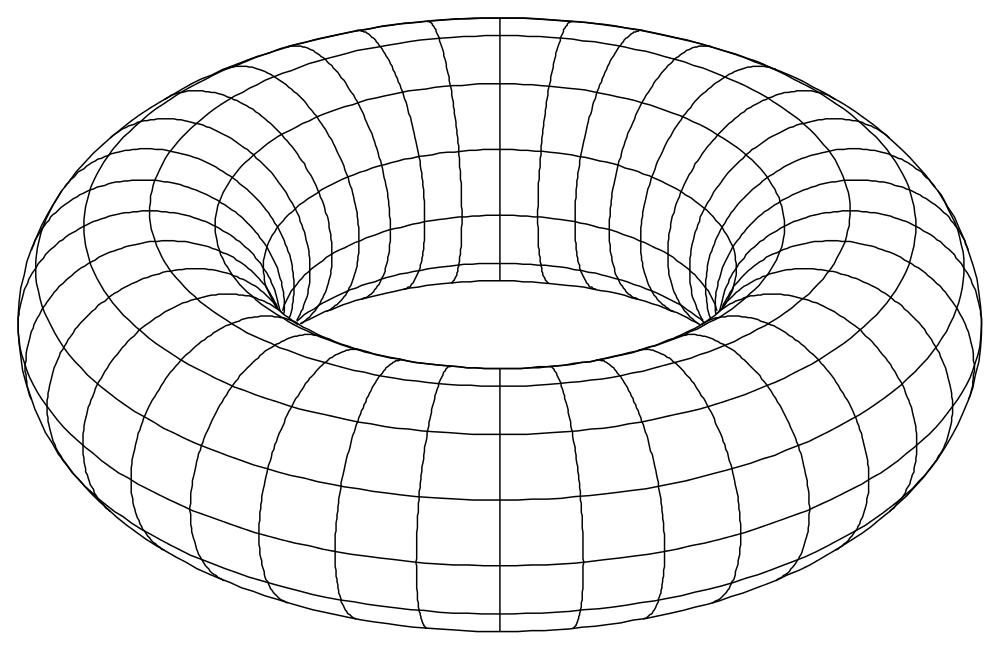
\includegraphics[scale = 0.15]{img/toro}
		\caption{Ilustración de un toro}
		\label{toro}
	\end{figure}
	Si consideramos la aplicación $\varphi:\R^2\to\R^4$ definida por:
	\[\begin{split}
	x&=\cos(2\pi x),\\
	y&=\sen(2\pi x),\\
	z&=\cos(2\pi y),\\
	t&=\sen(2\pi y).
	\end{split}\]
	Vamos a hacer pues una construcción similar a la ya vista para la circunferencia unidad. Nos queda un esquema del siguiente tipo:
	
	\[\xymatrix @C=0.5pc @R=0.5pc @L=-0.2pc {
		& \R^2\ar[rr] \ar[dd] & &
		\toro^2\subset\R^4 \\
		[0,1]^2 \ar@{}[ur]^*[@]{\subset} \ar[dr] \\
		& \R^2/\mathord{\sim}  \ar@{<->}[rruu]
	}\]
	
	En este caso, la relación de equivalencia inducida es (¡háganse las cuentas!):
	\[(x,y)\sim (x',y')\iff x-x'\in\Z,\;y-y'\in\Z\]
	y como dominio fundamental encontramos el cuadrado $[0,1]^2$.
	
	La demostración de que $\varphi$ es indentificación sigue la misma filosofía que la del ejemplo anterior, es decir, se basa en demostrar que es homeomorfismo local (no lo haremos aquí).
	
	Así pues queda demostrado que si cogemos un cuadrado y ``pegamos'' sus bordes tal y como indica la figura \ref{const_img_polfun_toro} obtenemos un espacio homeomorfo al toro, es decir a $\esfera^1\times \esfera^1$. Dicho formalmente $[0,1]^2/\mathord{\sim}$ es homeomorfo al toro plano.
	\end{exa}
	A menudo, los dominios fundamentales son representables mediante esquemas llamados \tbi[polígono fundamental]{polígonos fundamentales} (recortables ifantiles exóticos).
	
	La forma de entenderlos es que la relación de equivalencia ``pega'' los puntos de $A$ y de $B$ en el sentido que indican las flechas, como vemos en el ejemplo siguiente, que representa el toro que acabamos de describir:
	
	% Copiado de https://en.wikipedia.org/wiki/Fundamental_polygon . Querría hacer uno yo pero no ha dado tiempo.
	\begin{figure}[h!]
		\centering
		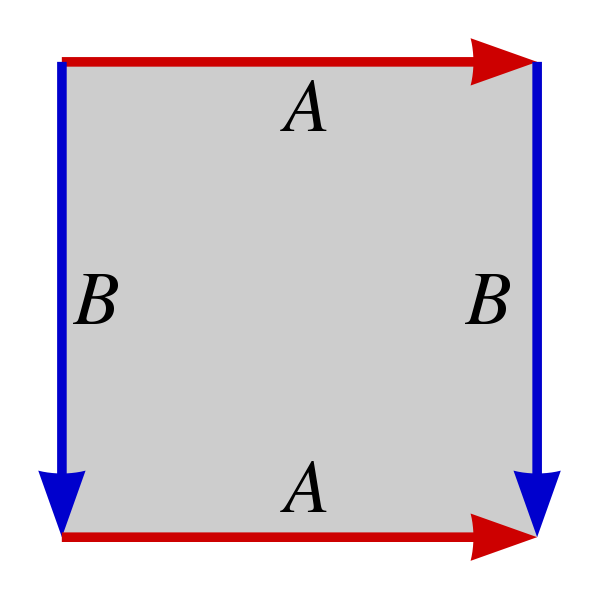
\includegraphics[scale = 0.1]{img/pol_fund_toro}
		\caption{Polígono fundamental de un toro plano}
		\label{const_img_polfun_toro}
	\end{figure}

En el siguiente ejemplo, vamos a ver varios homeomorfismos cociente importantes pero sin entrar en tantos detalles como en los ejemplos previos. Para familiarizarnos íntimamente con el espacio cociente, es un buen ejercicio mental tratar de visualizar cómo podemos deformar un objeto del ejemplo siguiente para transformarlo en otro homeomorfo. Al fin y al cabo, la homeomorfia, intuitivamente, es poder deformar sin romper, y los cocientes formalizan la noción de ``pegar'' puntos.
\begin{exa}[Otros espacios cociente interesantes]\
	\begin{enumerate}
		\item La esfera $\esfera^2$ se puede identificar con el disco unidad si la relación de equivalencia es la que hace que todos los puntos del borde (la circunferencia) estén relacionados entre sí y los demás, solo consigo mismos. De la misma forma, la podemos identificar con dos discos donde la relación de equivalencia ``pega'' los bordes.
		
		Por último, una esfera puede identificar con un polígono fundamental de la siguiente manera
		
		\begin{figure}[h!]
			\centering
			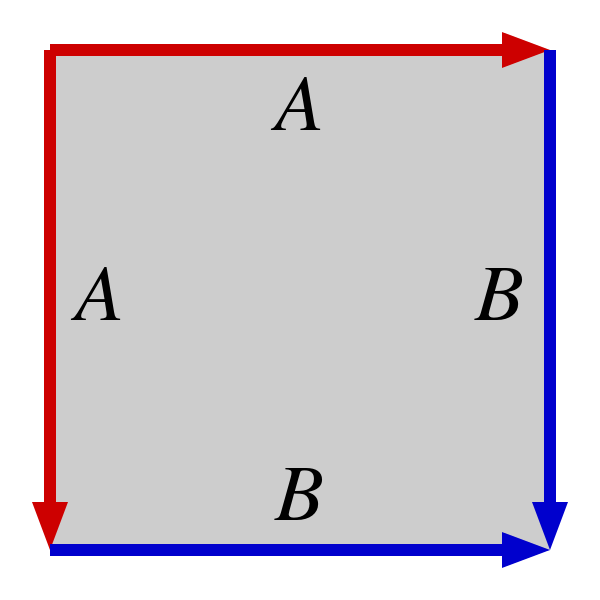
\includegraphics[scale = 0.1]{img/pol_fund_esfera}
			\caption{Polígono fundamental de la esfera.}
		\end{figure}
		
		\item Podemos identificar el plano proyectivo real $\proy^2$ con un disco y una banda de Möbius donde la relación de equivalencia ``pega'' los bordes (tiene su miga y no lo haremos aquí).
		
		También podemos identificarlo con una semiesfera en la que cada punto del borde es equivalente a su antípoda, o con una esfera completa en la que dos puntos están relacionados si y solo si son antipodales.
		
		Además, también admite una identificación como polígono fundamental
		
		\begin{figure}[h!]
			\centering
			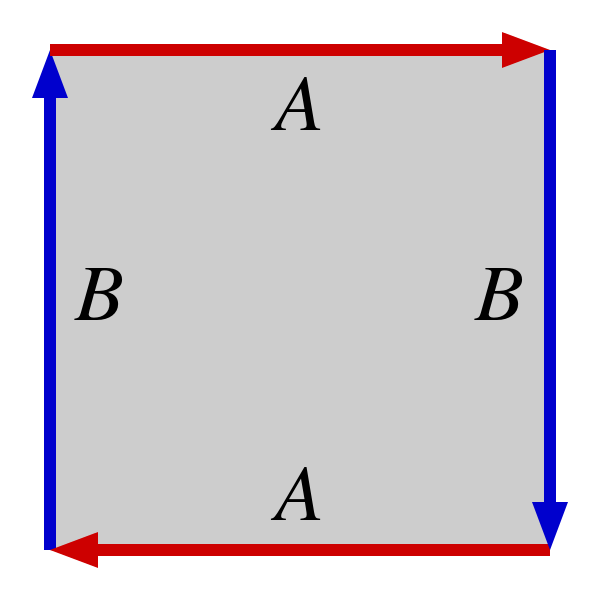
\includegraphics[scale = 0.1]{img/pol_fund_plano_proy}
			\caption{Polígono fundamental del plano proyectivo real.}
		\end{figure}
		
		\item Ya como colofón podemos definir como espacios con topología cociente dos objetos más.
		\begin{figure}[h!]
			\centering
			\subfigure[Banda de Möbius]{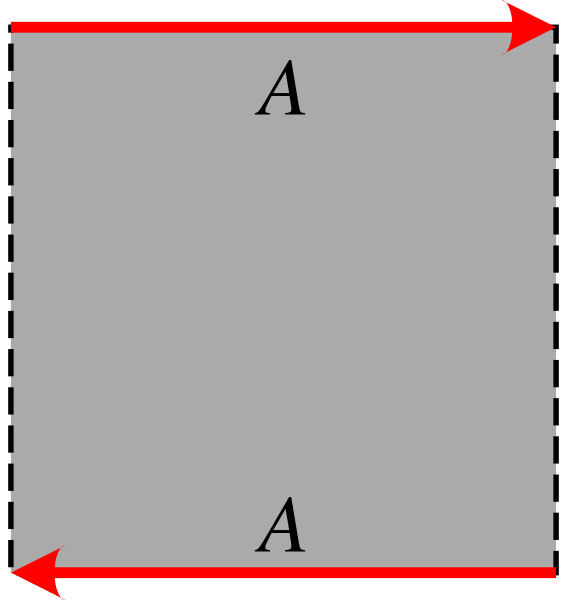
\includegraphics[scale = 0.09]{img/pol_fund_mobius}}
			\subfigure[Botella de Klein]{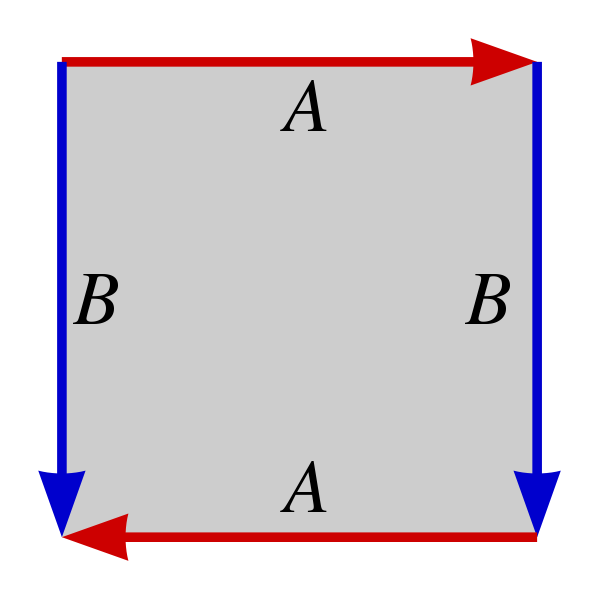
\includegraphics[scale = 0.1]{img/pol_fund_botella_klein}}
			\caption{Banda de Möbius y Botella de Klein}
		\end{figure}
	\end{enumerate}
	Esto es objetivamente bonito.
\end{exa}
\begin{obs}[Otro tipo de problema]
	\label{const_otroProb}
	Puede ocurrir que no tengamos ni idea de cual puede ser una posible identificación entre un espacio y otro pero si sepamos a qué cociente podría ser homeomorfo el espacio a estudiar, lo cual, a la postre puede ayudarnos a encontrar una identificación cuyo cociente inducido sea el candidato (y demostrar así la homeomorfía).
\end{obs}
\begin{exa}[Cilindro]
	Para ilustrar el problema descrito en la observación \ref{const_otroProb} vamos a imaginar que estamos en el jardín de infancia jugando con cartulinas, nosotros, que somos chavales avispados, sabemos que el cilindro se define como $\esfera^1\times[0,1]\subset\R^3$, pero nosotros sólo tenemos una cartulina, eso es $[0,1]^2$. De pronto se nos enciende la bombilla y decimos, ``¡anda coño!'' (Arquímedes hubiera dicho ``¡eureka!'') y comprobamos que si pegamos los bordes del cuadrado nos sale algo, así a ojo, muy parecido a un cilindro.
	
	Esta idea de pegar los bordes la podemos modelizar con la relación de equivalencia
	\[(x,y)\sim (x',y')\sii x-x'\in\Z\text{, }y=y'\]
	Visto con polígono fundamental
	\begin{figure}[h!]
		\centering
		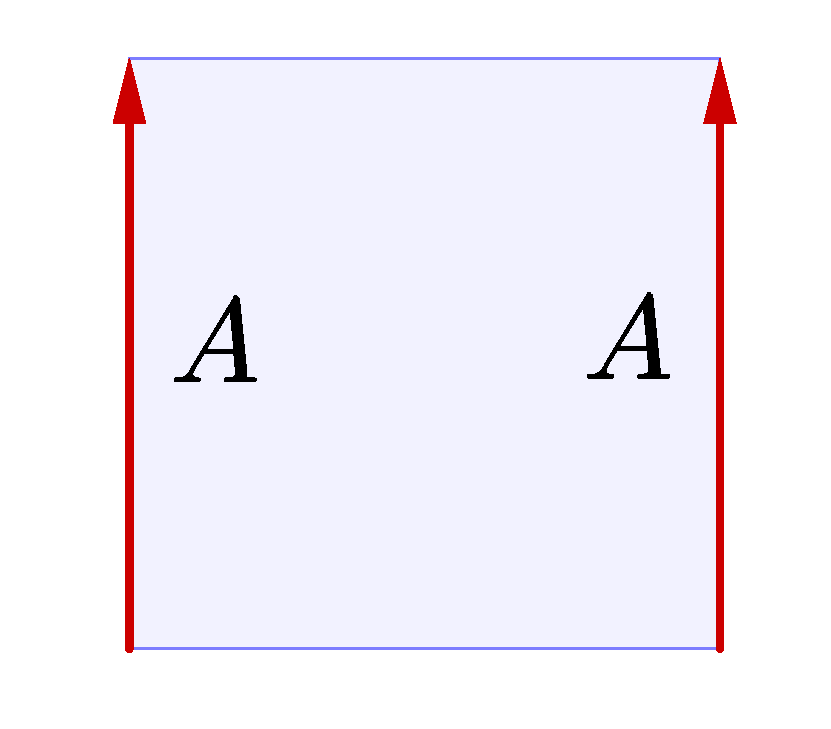
\includegraphics[scale = 0.15]{img/pol_fun_cilindro}
		\caption{Polígono fundamental del cilindro.}
	\end{figure}
	
	Dicho formalmente, estamos considerando el espacio cociente $[0,1]^2/\mathord{\sim}$ como candidato a ser homeomorfo al cilindro. Para demostrar que así es debemos encontrar una aplicación $\varphi:[0,1]^2\to\esfera^1\times[0,1]$ tal que su relación de equivalencia asociada sea $\sim$ y además sea identificación.
	
	Es claro que se debe cumplir $\varphi(0,y)=\varphi(1,y)=(x',y',z')$ y que $x'^2+y'^2=1$ para todo $y\in[0,1]$.
	
	Llegados a este punto más vale que se te ilumine la cabeza y te des cuenta de que una función trigonométrica te haría muy buen apaño. Por ejemplo
	\[\begin{split}
		\varphi: x'= & \cos(2\pi x)\\
		y' =& \sen(2\pi x)\\
		z' =& y
	\end{split}\]
	Esta función cumple trivialmente todas las propiedades requeridas. Es evidente que es sobreyectiva en $\esfera^1\times [0,1]$ además también es continua, y, no solo eso sino que es homeomorfismo local, con lo cual es abierta.
	
	En ningún momento hemos demostrado que ningunas de las aplicaciones vistas en ejemplos sean homeomorfismos locales (que parece ser la clave para demostrar que son abiertas y por tanto identificaciones), sin embargo lo hacemos porque más adelante veremos resultados potentes que nos permitirán demostrar este tipo de cosas de un plumazo.
	
	Bien, si damos por hecho eso, ya habríamos demostrado formalmente que $[0,1]^2/\mathord{\sim}$ es homeomorfo al cilindro, y, por tanto, podríamos ir a pedir una pegatina en forma de estrella, que nos la hemos ganado. 
\end{exa}
\section{Producto de espacios topológicos}
Una vez visto el caso del espacio cociente, pasamos ahora a realizar un desarrollo similar para otras construcciones como son los productos y sumas de espacios topológicos. Se va a realizar un procedimiento análogo en el desarrollo de las mismas al de la anterior sección.

Sean $(X_{i },\T_{i})^{1\le i\le r}$ espacios topológicos y sea $Y=\prod_i X_i$. Tomamos entonces 
\begin{equation}
Y=\prod_i X_i \stackrel{p_i^r}{\longrightarrow}(X_i,\T_i)
\end{equation}
Lo que buscamos en la construcción del espacio producto es dotar a $Y$ de la topología $\T$ más fina que haga continuas todas las aplicaciones $p_i^r$ para $1\le i\le r$. A dichas  $p_i^r$ las conoceremos a partir de ahora como \tbi[proyeccion@proyección]{proyecciones}.

De este modo, como queremos que $p_i^r$ sea continua  tenemos que para todo abierto $U_i\in \T_i$ deberá verificarse que $(p_i^r)^{-1}(U_i)=X_1\times\cdots\times U_i\times\cdots X_r$ (todos son los totales excepto en el caso de $X_i$) sea abierto. Es decir, que se cumpla $X_1\times\cdots\times U_i \times\cdots X_r\in \T$

Por lo tanto, vemos que por ser topología ha de verificarse que $(p_i^r)^{-1}(U_i)\cap (p_j^r)^{-1}(U_j)= X_1\cdots\times U_i \times\cdots\times U_j\times \cdots X_r$ sea parte de ella (intersección de abiertos).

Si tomamos ahora $ \{ U_1\times\cdots\times U_r : U_i\in \T_i \}$ veamos que es una base de la topología que pretendemos construir. Esto va a resultar evidente, ya que tan solo debemos comprobar para demostrarlo que al intersecar dos elementos cualesquiera de la base nos queda otro elemento de la base. 

Como dados $U_1\times\cdots\times U_r$ y $V_1\times\cdots\times V_r$ elementos de la base su intersección es $(U_1\cap V_1)\times\cdots\times (U_r\cap V_r)$ y como $(U_i\cap V_i)\in \T_i$, afirmamos que forma parte de la base por la definición de la misma.

Así, una vez que tenemos la base que va a caracterizar nuestra topología producto podemos afirmar que esta viene dada por $\T=\prod_i \T_i$.

\begin{defi}[Topología producto]
	Sean $(X_{i },\T_{i})^{1\le i\le r}$ espacios topológicos y sea $Y=\prod_i X_i$. Entonces se conoce como \tbitop[$\T_1\times\T_2$]{producto} a la topología $\T$ de $Y$ que viene dada por la base $ \{ U_1\times\cdots\times U_r : U_i\in \T_i \}$ (es decir, el producto de las topologías).
\end{defi}

Podemos formular, además, una propiedad universal del producto que caracteriza a esta topología:

\begin{lem}[Propiedad universal del producto]
	En la siguiente situación,
	\[\xymatrix{
		Y=\prod_i X_i \ar[r]^{p_i} & 
		(X_i,\T_i) \\
		(Z,\T') \ar[u]^{(f_1,\dots,f_n)=f} \ar[ru]_{p_i\circ f=f_i} &
	}\]
	tenemos la \tbi[propiedad universal!del producto]{propiedad universal del producto} que caracteriza la continuidad de $f$, diciendo que esta será continua si y solo si $f_i=p_i^r\circ f$ son continuas para todo $i$.
	
	\begin{proof}
		Vemos que si $f$ es continua, como $p_i^r$ son continuas, tenemos que $f_i$ también lo será al ser composición de estas.
		
		Por otro lado, tenemos que dado $W=\prod_iU_i$ abierto en $X$, tenemos que $f^{-1}(W)=\bigcap_i f_i^{-1}(U_i)$ será abierto dado que los $f_i^{-1}(U_i)$ son abiertos por ser $f$ continua. Así, como hemos probado que la imagen inversa de abiertos es abierta, tenemos que $f$ es continua.
	\end{proof}
\end{lem}

Veamos ahora que la propiedad universal caracteriza la topología.

\begin{prop}
	Si $(Y,\T_Y)$ cumple la propiedad universal del producto, entonces $\T_Y = \prod\T_i $
\end{prop}
\begin{proof}
	Vamos a demostrarlo por doble contención y haciendo algún cambalache con la identidad.
	Empecemos con un diagrama para aclarar las ideas.
	\[\xymatrix{
		(Y,\T_Y) \ar[r]_{p_{r_i}}^{p_i} & 
		(X_i,\T_i) \\
		(Y,\T_Y) \ar[u]^{\text{id}} \ar[ru]_{p_{r_i} = p_{r_i} \circ \text{ id}} &
	}\]
	Como la topología $\T_Y$ cumple la propiedad universal y la aplicación identidad es continua, tenemos que $p_{r_i}$ es continua. Luego por finura $ \prod\T_i \subset \T_Y$.
	
	Ahora razonamos con este diagrama:
	\[\xymatrix{
		(Y,\T_Y) \ar[r]_{p_{r_i}}^{p_i} & 
		(X_i,\T_i) \\
		(Y,\prod\T_i) \ar[u]^{\text{id}} \ar[ru]_{p_{r_i} = p_{r_i} \circ \text{ id}} &
	}\]	
	Como por construcción $p_{r_i}$ es continua, entones id es continua. Esto solo ocurre si $\T_Y \subset \prod\T_i$. 	
\end{proof}

Vamos a ver ahora una serie de proposiciones relacionadas con la topología producto, las cuales a pesar de resultar sencillas de comprobar nos proporcionan resultados interesantes.

\begin{prop}
	Las proyecciones son abiertas.
	
	\begin{proof}
		Sea $W$ abierto en el espacio producto, veamos que $p_i^r(W)$ es abierto.
		
		Nos basta con comprobarlo con los abiertos de la base, es decir, para los elementos de la forma $ U_1\times\cdots\times U_r : U_i\in \T_i$.  Como  $p_i^r(U_1\times\cdots\times U_r)=U_i$ es abierto podemos concluir la demostración.
	\end{proof}
\end{prop}


\begin{prop}
	La aplicación $f : X_i\to\{a_1\}\times\cdots\times X_i\times\cdots\times \{a_r\}\subset X_1\times\cdots\times X_r$ tal que $x\mapsto (a_1,\dots,x,\dots,a_r)$ es una inmersión.
	
	\begin{proof}
		Evidentemente, f es biyectiva. Por otra parte, $f$ es la aplicación $(k_1,\dots,id,\dots,k_r)$ continua, por serlo la identidad.
		Además, $f^{-1} = p_{r_i}\restriction_{\{a_1\}\times\dots\times X_i \times \dots \times\{a_r\}}$ es continua por serlo las proyecciones. Luego f es homeomorfismo.
	\end{proof}
\end{prop}

\begin{obs}[Consecuencias]
	La topología de $\{a_1\}\times\dots\times X_i \times \dots \times\{a_r\}$ es exactamente la de $X_i$. Esto constituye un truco para comprobar si una topología es una topología producto.
\end{obs}
	

Ahora pasamos a ver si somos capaces de construir bases más sencillas para nuestra topología producto, es decir, conformadas por menos abiertos. Igualmente, veremos el modo de construcción de bases de entornos en el espacio producto. No vamos a probar que sean bases realmente en ninguno de los dos casos ya que en ambos casos va a resultar muy sencillo aplicando la caracterización de base, dejándose como ejercicio para el lector de cara al repaso de la misma.
\begin{enumerate}
	\item Dado el espacio producto $(\prod_iX_i,\prod_i\T_i)$ tenemos que: \[\B=\{W_i\times\cdots\times W_r:W_i\in \B_i \text{ base de }\T_i\}\] es base de entornos del mismo.
	\begin{proof}
		Sea $\U \in \T$. Podemos descomponerlo como sigue $\U =U_1 \times \dots \times U_r $ con $U_i \in \T_i$ y $U_i = \bigcup_j W_{ij}$ con $W_{ij} \in \B_i$. Sea $x \in \U$. Entonces $x \in \W_{1j} \times \dots \times W_{rj} \subset \bigcup_j W_{1j} \times \dots \times \bigcup_j W_{rj} = U_1 \times \dots \times U_r$. Haciendo este procedimiento para cada punto se sigue el resultado.
	\end{proof}

	\item Dado el espacio producto $(\prod_iX_i,\prod_i\T_i)$ y $(a_1,\dots,a_r)\in\prod_iX_i$ tenemos que: \[\V_{(a_1,\dots,a_r)}=\{V_{a_1}\times\cdots\times V_{a_r}:W_i\in \V_{a_i} \text{ base de entornos en } \T_i\} \] es base de entornos del mismo.
\end{enumerate}

Por último, algunas observaciones útiles sobre la topología de los productos son
\begin{prop}[Adherencia]
	Sean $X_i$ espacios topológicos y $A_i$ subconjuntos de $X_i$. Tenemos que
	\[Adh(A_1 \times \dots \times A_r) = Adh(A_1) \times \dots \times Adh(A_r)\]
\end{prop}
\begin{proof}
	 Por una parte tenemos que $x \in Adh(A_1 \times \dots \times A_r) \iff$ dado un entorno $U_1 \times \dots \times U_r$ de $x$, dicho entorno corta a $A_1 \times \dots \times A_r$.
	 Por otra parte, $x \in  Adh(A_1) \times \dots \times Adh(A_r) \iff \ \forall U_1 \times \dots \times U_r $ se cumple que $U_i \cap A_i \neq \emptyset \ \forall i$.
	 Finalmente, gracias a la siguiente propiedad $(U_1 \times \dots \times U_r) \cap (A_1 \times \dots \times A_r) = (U_1 \cap A_1) \times \dots \times (U_r \cap A_r)$ se llega al resultado.
\end{proof}

\begin{prop}[Cerrados]
	Sean $X_i$ espacios topológicos y $A_i$ subconjuntos de $X_i$. Tenemos que
	$A_1 \times \dots \times A_r$ es cerrado $\iff A_i$ es cerrado $\forall i$.
\end{prop}
\begin{proof}
	Veamos que si $A_i$ es cerrado $\forall i$ entonces $A_1 \times \dots \times A_r$ es cerrado. Basta ver que $A_1 \times \dots \times A_r$ coincide con su adherencia, que por la proposición anterior coincide con $Adh(A_1) \times \dots \times Adh(A_r)$, que a su vez es $A_1 \times \dots \times A_r$, pues cada $A_i$ coincide con su adherencia por ser cerrado.
	La otra implicación se deja al lector.
\end{proof}	

		
\section{Suma}
Vamos a ver como última la construcción la suma, la cual gracias al desarrollo previo de los casos anteriores va a resultar de fácil comprensión para el lector. La idea de esta construcción va a ser la de realizar copias de objetos a distintas ``alturas'' (como si los colocáramos en estantes). 

Como antes, vamos a comenzar viendo las propiedades que debe cumplir la topología que caracterice nuestro espacio para luego pasar a construirla.

Dados los espacios $(X_i, \T_i)^{1\le i \le r}$ con sus correspondientes topologías, construimos el espacio suma como
\begin{equation}
(X_i, \T_i)\stackrel{j_i}\longrightarrow Y=\sum_{i=1}^rX_i=\bigcup_{i=1}^r\{i\}\times X_i
\end{equation}
Conviene resaltar que, como podemos observar, las copias de los distintos espacios $X_i$ en la suma será distinta, dado que a cada una le corresponderá un elemento $i$ distinto.

Ahora bien, nuestro objetivo en esta construcción será el de crear la topología $\T$ más fina en $Y$ de modo que haga las $j_i$ continuas. Las funciones $j_i$ las llamaremos \tbi{inclusiones}.

Por definición de continuidad, podemos (y debemos, ya que buscamos que sea la más fina) incluir en $\T$ todos los conjuntos de $Y$ cuya inversa sea abierta.
De este modo, también incluiremos $\{i\}\times X_i$ dado que $j^{-1}(\{i\}\times X_i)=X_i$ que es abierto en $\T_i$.

Ahora construimos la topología que tiene como base $\B=\{\{i\}\times U_i:U_i\in\T_i\}$ comprobemos que está bien definida y que es realmente base.
\begin{equation}
(\{i\}\times U_i)\cap(\{j\}\times U_j)=
\left\{ \begin{array}{lcc}
\{i\}\times(U_i\cap U_j)\in\T &   si  & i=j \\
\\  \emptyset\in\T& si & i\neq j 
\end{array}
\right.
\end{equation}
Como podemos ver, ambos casos verifican que la intersección está contenida en $\T$ como debiamos demostrar para ver que es base del mismo.
Así, podemos definir:
\begin{defi}[Topología suma]
	Dados los espacios con sus correspondientes topologías $(X_i, \T_i)^{1\le i \le r}$ y el espacio suma $Y=\sum_{i=1}^rX_i$, construimos la \tbitop{suma} como aquella topología que tiene como base $\B=\{\{i\}\times U_i:U_i\in\T_i\}$.
\end{defi}

Una vez vista su definición, veamos ahora un resultado fundamental acerca de la topología suma que no va a ser otra que la siguiente propiedad universal:

\begin{lem}[Propiedad universal de la suma]
	En la siguiente situación:
	\[\xymatrix{
		X \ar[rd]^f & \\
		X_i \ar[u]^{j_i} \ar[r]_{f_i} &
		Y
	}\]
	tomando en $X_i$ las topologías $\T_i$ y siendo $(Y,\T)$, tenemos la siguiente \tbi[propiedad universal!de la suma]{propiedad universal de la suma} que caracteriza la continuidad de $f$, diciendo que esta será continua si y solo si  $f_i=j_i\circ f$ son continuas para todo $i$.
	
	\begin{proof}
		Vemos que si $f$ es continua, como $j_i$ son continuas, tenemos que $f_i$ también lo será al ser composición de estas.
		
		Por otro lado, tenemos que dado que $(Y,\T)$ como hemos visto en la construcción de la topología suma $T$ es un recubrimiento abierto y continuo en cada uno de los $X_i$, tenemos que al ser continuo cada $f_i$ en $X_i$ también lo será $f$.
	\end{proof}
\end{lem}

Resulta importante indicar que como se desprende de la demostración (segunda implicación) la propiedad universal no solo nos va a caracterizar la función $g$, sino que nos permite caracterizar también la topología suma (si no se cumple la propiedad podemos asegurar que no estamos trabajando en esta). 

\begin{obs}
	Veamos por último un par de observaciones sobre esta topología que pueden resultar interesantes de cara a conocer el mecanismo de la misma.
	\begin{enumerate}
	\item Como hemos visto, $\{i\}\times X_i\subset\sum_j X_j$ siendo $\{i\}\times X_i$ abierto. Veamos que también es cerrado.
	
	Dado que $\sum_j X_j\setminus \{i\}\times X_i=\bigcup_{j\ne i }X_j$ es abierto, lo tenemos.
	
	\item Las inclusiones $X_l\stackrel{j_l}\longrightarrow\sum_iX_i$ son inmersiones abiertas y cerradas. Esto lo dejamos como ejercicio al lector, es un ejercicio sencillo pero puede resultar útil como repaso del modo de construcción de la topología suma realizado previamente en el apartado. \qedhere
\end{enumerate}
\end{obs}
